\hypertarget{semicircle_8cpp}{
\subsection{/home/luiggi/Documents/Research/Meshless\_\-RBF/NEW/RBFSoft/examples/01TestKnots/semicircle.cpp File Reference}
\label{semicircle_8cpp}\index{/home/luiggi/Documents/Research/Meshless\_\-RBF/NEW/RBFSoft/examples/01TestKnots/semicircle.cpp@{/home/luiggi/Documents/Research/Meshless\_\-RBF/NEW/RBFSoft/examples/01TestKnots/semicircle.cpp}}
}
Testing the \hyperlink{classSemiCircleKnots}{SemiCircleKnots} class.  




\subsubsection{Detailed Description}
Testing the \hyperlink{classSemiCircleKnots}{SemiCircleKnots} class. 

In this example some features of the class \hyperlink{classSemiCircleKnots}{SemiCircleKnots} are tested. Particularly the function \hyperlink{classKnots_dd136cbe2ce6474885aab4829576472b}{Knots::findNeighbors()} is used to find the neighborhood of a target point. \begin{Desc}
\item[Input]The {\tt inputSemiCircle} file contains the input data required for this program: {\tt r1} and {\tt r2} Radii for defining the semicircle; {\tt t1} and {\tt t2} Angles for defining the semicircle; {\tt Nr} number of points in R; {\tt Nt} number of points in theta; {\tt rtype} knots distribution (0 unif, 1 rand, 2 rand unif); {\tt ep} degree of randomness. \end{Desc}
\begin{Desc}
\item[Output]{\tt xyzSemi.dat} coordinates of random points; {\tt tarSemi.dat} the target point; {\tt neiSemi.dat} list of neighbors of the target. \end{Desc}
\begin{Desc}
\item[Post-procesing]You can plot the results using the next command in gnuplot: 

\footnotesize\begin{verbatim}
    % gnuplot> p "neiSemi.dat" w lp, "xyzSemi.dat" w p, "tarSemi.dat" w p \end{verbatim}
\normalsize
 \end{Desc}
 \begin{Image}
\begin{center}
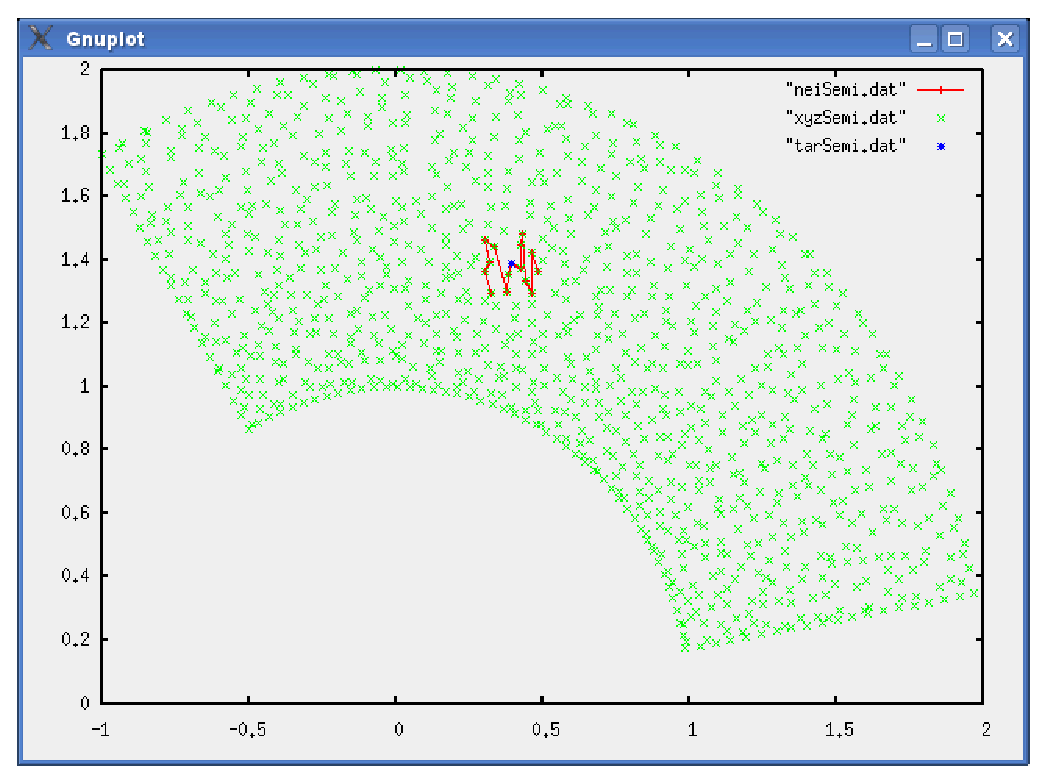
\includegraphics[width=5cm]{semtest}\caption{Knots, target and neighborhood.}
\end{center}
\end{Image}


\begin{Desc}
\item[Author:]Luis M. de la Cruz \mbox{[} Thu Sep 6 14:35:41 BST 2007 \mbox{]} \end{Desc}


Definition in file \hyperlink{semicircle_8cpp-source}{semicircle.cpp}.